%  Time 01: 
%    Gate 00 toffoli(j0,j1,j2) 
%  Time 02: 
%    Gate 01 X(j0) 
%  Time 03: 
%    Gate 02 c-U(j2,j3,j0,j1) 
%  Time 04: 
%    Gate 03 H(j2) 
%    Gate 04 measure(j3) 

% Qubit circuit matrix:
%% j0: gAxA, gBxA, gCxA, n  , n   
% j1: gAxB, n  , gCxB, n  , n   
% j2: gAxC, n  , gCxC, gDxC, n   
% j3: n  , n  , gCxD, gDxD, N   

\documentclass[11pt]{article}
%
% File:   xyqcirc.tex
% Date:   14-Mar-04
% Author: I. Chuang <ichuang@mit.edu>
%
% Definitions for producing quantum circuits with XYPIC in latex
%
% $Log: xyqcirc.tex,v $
% Revision 1.17  2004/03/25 05:01:23  ike
% discard and slash
%
% Revision 1.16  2004/03/25 04:58:42  ike
% added discard, and variable width dmeter
%
% Revision 1.15  2004/03/24 23:43:33  ike
% \dmeter and \sq
%
% Revision 1.14  2004/03/24 20:29:40  ike
% added \t for swap
%
% Revision 1.13  2004/03/24 17:52:16  ike
% removed \w from \gspace
%
% Revision 1.12  2004/03/24 16:38:34  ike
% added small space before |0> for \z
%
% Revision 1.11  2004/03/24 16:23:11  ike
% added \z
%
% Revision 1.10  2004/03/24 16:19:11  ike
% added multiple qubit operations
%
% Revision 1.9  2004/03/24 03:03:44  ike
% typo
%
% Revision 1.8  2004/03/24 02:50:09  ike
% added qv
%
% Revision 1.7  2004/03/24 00:07:34  ike
% add \m matrix op
%
% Revision 1.6  2004/03/23 23:13:10  ike
% misc
%
% Revision 1.5  2004/03/23 23:12:42  ike
% works now
%
% Revision 1.4  2004/03/23 22:22:34  ike
% ifthen also failes - because xymatrix entries in \save...\restore
%
% Revision 1.3  2004/03/23 21:34:36  ike
% no q/c wire switching
%
% Revision 1.2  2004/03/23 21:25:29  ike
% classical qo quantum wire switching try
%
% Revision 1.1  2004/03/23 21:01:46  ike
% Initial revision
%

%%%%%%%%%%%%%%%%%%%%%%%%%%%%%%%%%%%%%%%%%%%%%%%%%%%%%%%%%%%%%%%%%%%%%%%%%%%%%
% preliminaries

\usepackage{graphicx}

\usepackage[frame,line,arrow,matrix,tips]{xy}	% all that is usually necessary
\CompilePrefix{xygui-}
\makeindex
\pagestyle{empty}

\setlength{\oddsidemargin}{-0.5in}	% 1.25in left margin 
\setlength{\evensidemargin}{-0.5in}	% 1.25in left margin (even pages)

\setlength{\topmargin}{0.0in}		% 1in top margin
\setlength{\textwidth}{6.25in}		% 6.0in text - 1.25in rt margin
\setlength{\textheight}{8.6in}		% Body ht for 1in margins
\addtolength{\topmargin}{-\headheight}	% No header, so compensate
\addtolength{\topmargin}{-\headsep}	% for header height and separation

\begin{document}

\thispagestyle{empty}

%%%%%%%%%%%%%%%%%%%%%%%%%%%%%%%%%%%%%%%%%%%%%%%%%%%%%%%%%%%%%%%%%%%%%%%%%%%%%
% wires

\def\w{\ar@{-}[l]}
\def\W{\ar@{=}[l]}

%%%%%%%%%%%%%%%%%%%%%%%%%%%%%%%%%%%%%%%%%%%%%%%%%%%%%%%%%%%%%%%%%%%%%%%%%%%%%
% labels

% simple label
\def\A#1{\save []="#1" \restore}

%%%%%%%%%%%%%%%%%%%%%%%%%%%%%%%%%%%%%%%%%%%%%%%%%%%%%%%%%%%%%%%%%%%%%%%%%%%%%
% single qubit operations

\def\op#1{*+[F]{\rule[-0.2ex]{0ex}{2.1ex}#1}}	% operator in box
\def\b{*={\bullet}}
\def\o{*={\oplus}}
\def\t{*={\times}}				% for swap gate
\def\sq{*=<6pt,6pt>[F]{}}			% square, for controlled-phase
\def\m#1{\left[\matrix{#1}\right]}		% matrix shortcut
\def\z{*+[]{\rule[-0.2ex]{0ex}{2.1ex}~|0\>}}	% re-init to |0>
\def\discard{*[]{\rule[-0.2ex]{0.75pt}{2.1ex}~}}	% vertical ``|''
\def\slash{*={/}}				% slash for wire bundles

%%%%%%%%%%%%%%%%%%%%%%%%%%%%%%%%%%%%%%%%%%%%%%%%%%%%%%%%%%%%%%%%%%%%%%%%%%%%%
% nop's

\def\N{*-{}\W}
\def\n{*-{}\w}

%%%%%%%%%%%%%%%%%%%%%%%%%%%%%%%%%%%%%%%%%%%%%%%%%%%%%%%%%%%%%%%%%%%%%%%%%%%%%
% misc definitions

\def\>{\rangle}
\def\<{\langle}
\def\ua{\uparrow}

% measurement box
\def\meter{*+[]{\put(-3,0){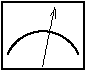
\includegraphics[scale=.5]{meter}}~~~~}%
		\ar@{-}[l]}

%%%%%%%%%%%%%%%%%%%%%%%%%%%%%%%%%%%%%%%%%%%%%%%%%%%%%%%%%%%%%%%%%%%%%%%%%%%%%
% qubit names (and also revert to qubit wires, vs, cbit wires)

\def\q#1{*+{\rule[-0.2ex]{0ex}{2.1ex}|#1\>}}
\def\qv#1#2{*+{\rule[-0.2ex]{0ex}{2.1ex}|#1\>=|#2\>}}
	
%%%%%%%%%%%%%%%%%%%%%%%%%%%%%%%%%%%%%%%%%%%%%%%%%%%%%%%%%%%%%%%%%%%%%%%%%%%%%
% multiple qubit gates

% utulity text box for figuring out width of things
\newbox{\sbox}

% empty space of width determined by the text argument
\def\gspace#1{*+{\rule[-0.2ex]{0ex}{2.1ex}%
	\setbox\sbox=\hbox{$#1$}%
	\hspace*{\wd\sbox}}}
	
% n-qubit operation #1=box label, #2=number of qubits (eg d=2 qubits, ddd=4)
\def\gnqubit#1#2{\gspace{#1}
		 \save [].[#2]!C="qq"*[F]\frm{}\restore
		 \save "qq"*[]{#1} \restore}

% two-qubit operation
\def\gtwo#1{\gnqubit{#1}{d}}

% two-qubit operation
\def\gthree#1{\gnqubit{#1}{dd}}

%%%%%%%%%%%%%%%%%%%%%%%%%%%%%%%%%%%%%%%%%%%%%%%%%%%%%%%%%%%%%%%%%%%%%%%%%%%%%
% ``D'' style measurement gate a-la-cleve, at Michael Nielsen's request

\def\dmeterwide#1#2{*{\xy <0pt,-8pt>;<0pt,8pt> **@{-};
		    <0pt,-8pt>;<#2,-8pt> **@{-} ;
		    <0pt, 8pt>;<#2, 8pt> **@{-} ;
		    <#2,0pt>-<5pt,0pt>*{#1} ;
		    <#2,0pt>*\cir<8pt>{r_l}\endxy}}

\def\dmeter#1{\dmeterwide{#1}{12pt}}

%%%%%%%%%%%%%%%%%%%%%%%%%%%%%%%%%%%%%%%%%%%%%%%%%%%%%%%%%%%%%%%%%%%%%%%%%%%%%


% definitions for the circuit elements 
\def\gAxA{\b\w\A{gAxA}}
\def\gAxB{\b\w\A{gAxB}}
\def\gAxC{\o\w\A{gAxC}}
\def\gBxA{\op{X}\w\A{gBxA}}
\def\gCxC{\b\w\A{gCxC}}
\def\gCxD{\b\w\A{gCxD}}
\def\gCxA{\b\w\A{gCxA}}
\def\gCxB{\op{U}\w\A{gCxB}}
\def\gDxC{\op{H}\w\A{gDxC}}
\def\gDxD{\meter\w\A{gDxD}}

% definitions for bit labels and initial states 
\def\bA{ \q{j_{0}}}
\def\bB{ \q{j_{1}}}
\def\bC{ \q{j_{2}}}
\def\bD{ \q{j_{3}}}

% The quantum circuit as an xymatrix 
\xymatrix@R=5pt@C=10pt{ 
    \bA & \gAxA &\gBxA &\gCxA &\n   &\n  
\\  \bB & \gAxB &\n   &\gCxB &\n   &\n  
\\  \bC & \gAxC &\n   &\gCxC &\gDxC &\n  
\\  \bD & \n   &\n   &\gCxD &\gDxD &\N  
% 
% Vertical lines and other post-xymatrix latex % 
\ar@{-}"gAxC";"gAxA"\ar@{-}"gAxC";"gAxB"\ar@{-}"gCxB";"gCxC"\ar@{-}"gCxB";"gCxD"\ar@{-}"gCxB";"gCxA"}
 
\end{document}